\documentclass{article}
\usepackage[utf8]{inputenc}
\usepackage[english]{babel}
\usepackage{graphicx}
\usepackage{float}
\usepackage[dvipsnames]{xcolor}
\usepackage[section]{placeins}
\pagenumbering{roman}


\title{EECS 31L - Final Project}
\author {
\textbf{Um Group}
\\
\\Kathy Nguyen (49131012), Joshua Park (25729974), Aina Tancinco (66726318), 
\\ Nicole Thai (55729939), Amy Yee (55246967)
} % end author
\date{December 11, 2017}

\begin{document}

\maketitle

\section{Introduction}
In this project, we design and implement a Processor for the RISC-V instruction set architecture. The processor contains three submodules that parse periodic inputs. The output then communicates with the BASYS-3 board to display a 4-bit number on the board's 7-segment display.

\subsection{Processor Block Diagram}
% BLOCK DIAGRAM of the entire processor and mention input/output ports of each block on the block diagram,
\begin{figure}[H]
  \centering
    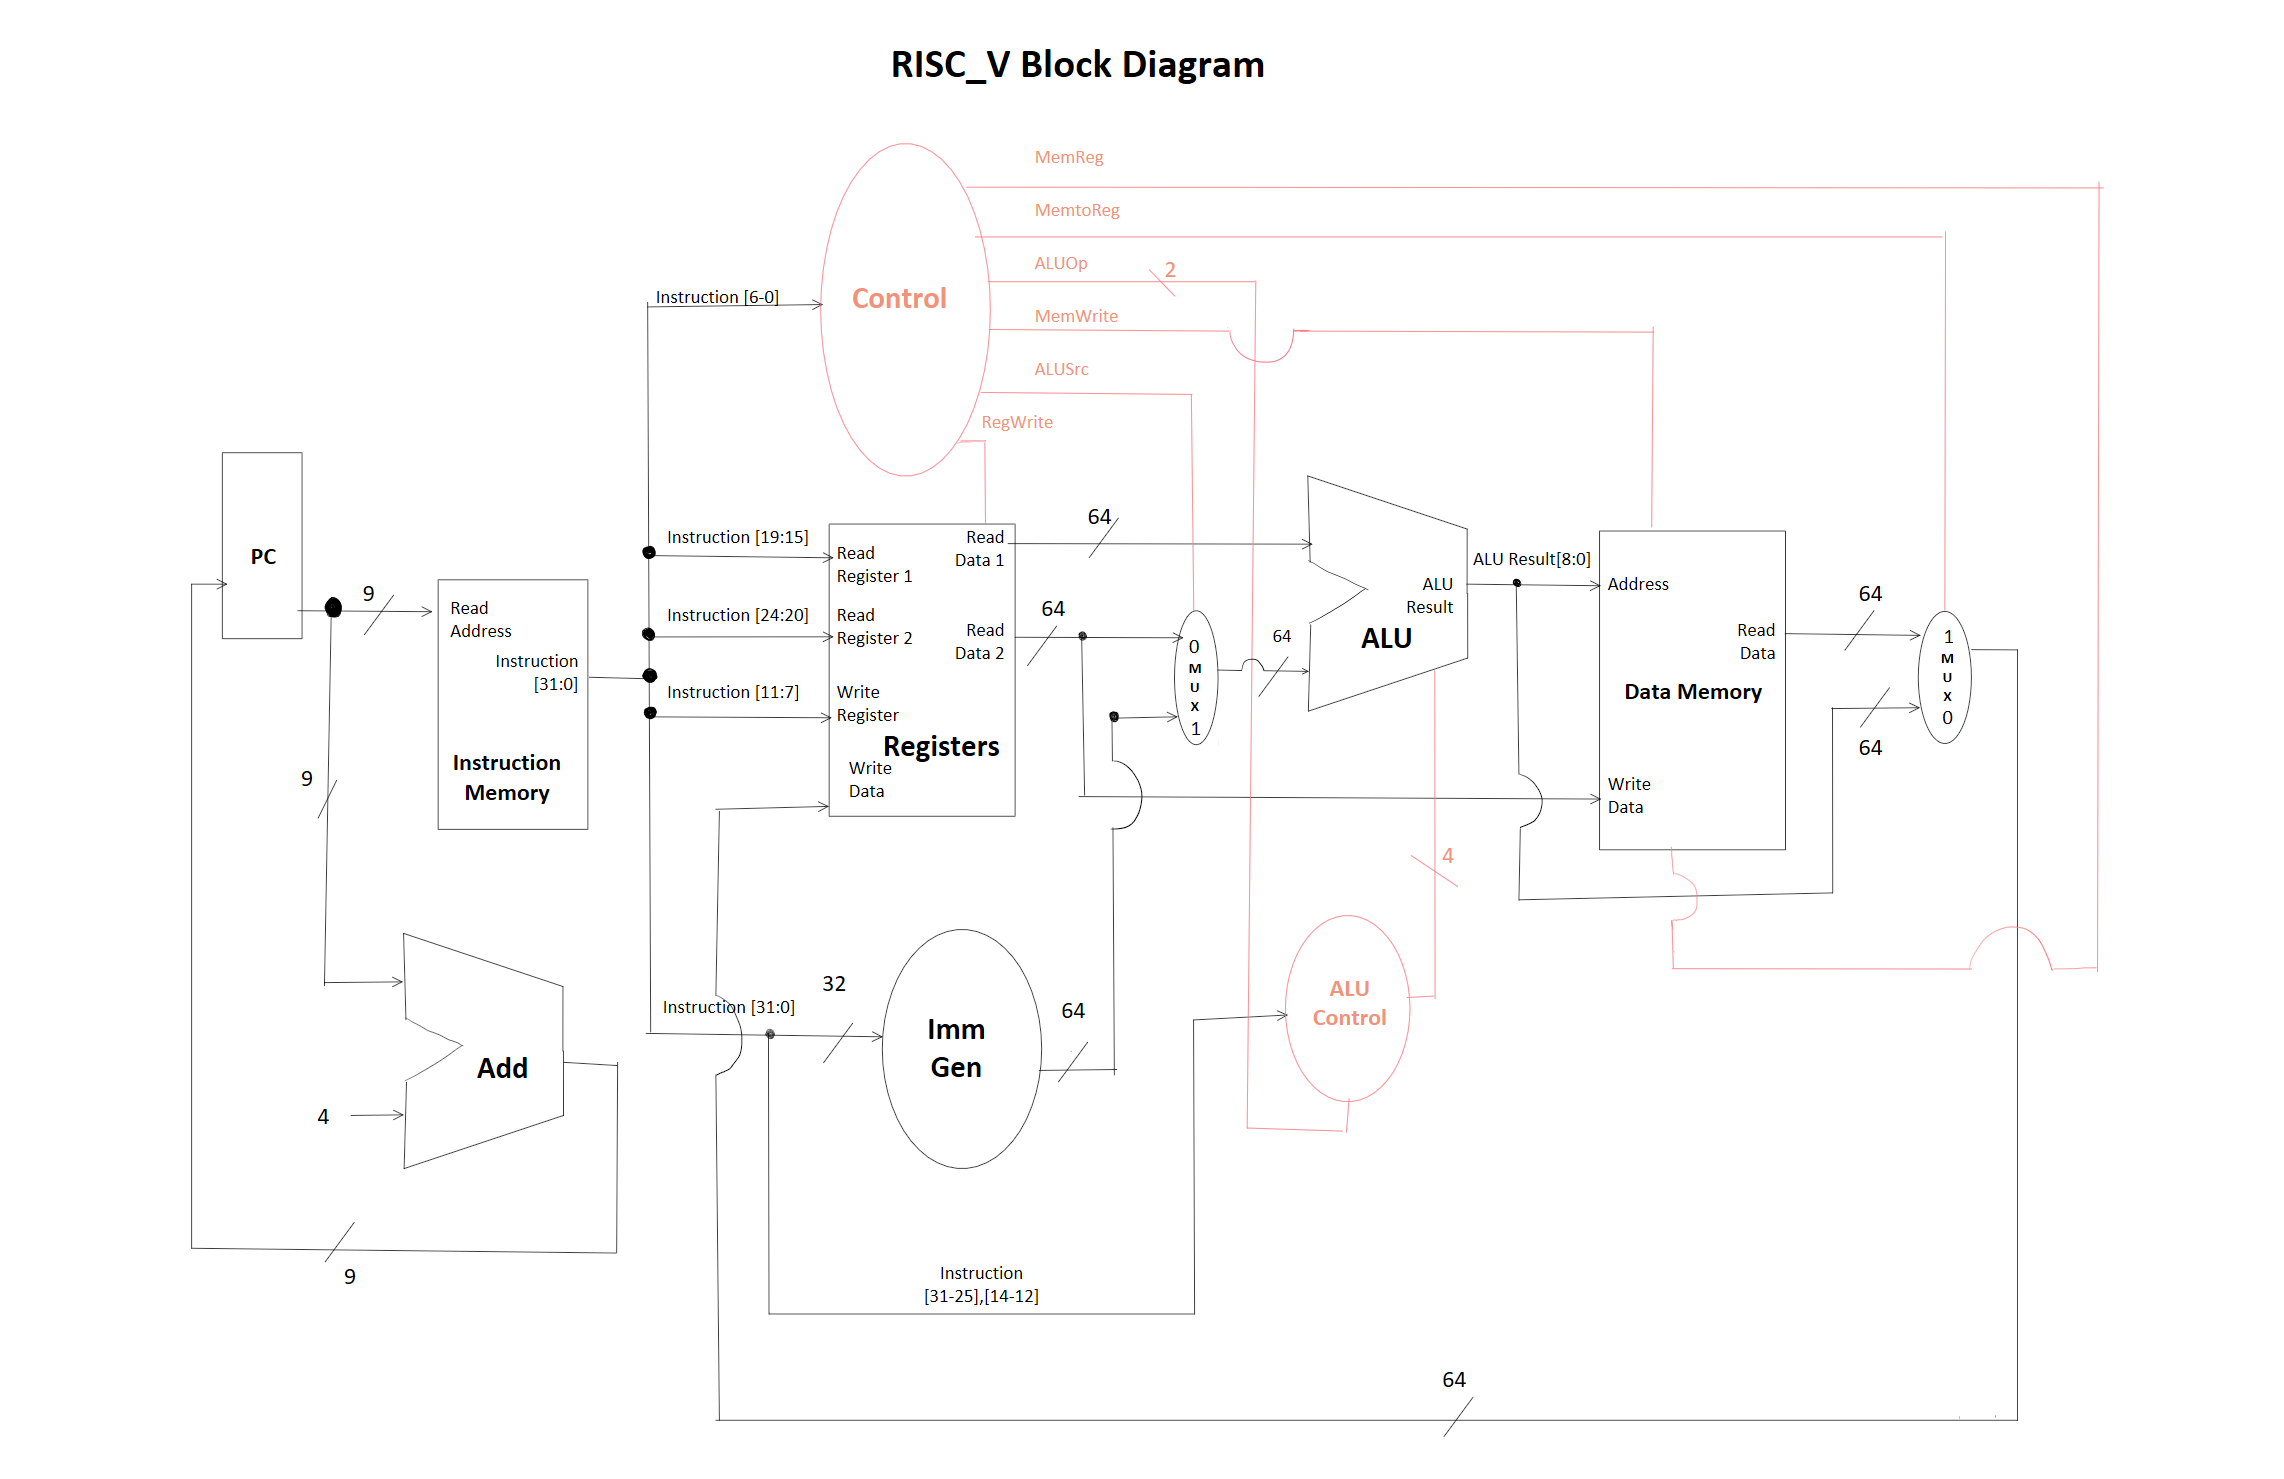
\includegraphics[width=\textwidth]{RISC_V.png}
  \caption{A RISC-V specific Processor.}

\end{figure}

\section{RISC-V}
The RISC-V processor contains three submodules built in previous labs: the controller, the ALU controller, and the datapath. To achieve this connection, a RISC-V module instantiates these three submodules. Additional wires provided by the RISC-V module - RegWrite, ALUSrc, MemRead, MemWrite, and MemtoReg - connect the controller to the datapath.  The wire ALUOp connects the controller to the ALU controller. Lastly, the ALU Control Code connects the ALU controller to the datapath. Inputs include a clock and asynchronous reset. The output of the RISC-V processor is the final result of the ALU. \\

An test bench ensures the modules are properly instantiated and the overall processor returns expected output. The test bench module tb\_RISC\_V instantiates to input and output values of the RISC\_V module and feeds input signals to the instantiated module. Comparing the resulting output waveforms with the expected outputs allow the designer to verify whether the design is correct under multiple test cases.


\section{Data Path}
The Data Path module instantiates seven submodules: Program Counter, Immediate Generator, Instruction Memory, Register File, ALU, Data Memory, and Multiplexer. 

\subsection{Program Counter}

The purpose of the Program Counter (PC) is to select the starting addresses that storing a single instruction for instruction memory to read. PC is only byte addressable which is equivalent to 8 bits. In addition, the PC sends the starting address of the next 4 bytes containing a 32 bit instruction. As a result, we have to include an adder to make 4 bytes into a clump of 32 bits. We add by 4 to the PC to access the next starting address of another instruction. The flip flop is also necessary for the PC so that the PC stores the next address location until the clock is enabled.The adder would produce new instructions every 4 byte or 32 bits from the 0-128 addresses.

\subsection{Immediate Generator}
The Immediate Generator (ImmGen) receives a 32-bits instruction from the Instruction Memory. The least seven significant bits of the opcode determine whether the instruction is R-type, I-type, or S-type. The three different types interpret the immediate differently. R-type does not contain immediate data types. On the other hand, I-type instructions interpret the 12 most significant bits as the immediate while S-type instructions interpret the 7 most significant bits as the immediate. After interpreting the immediate, the ImmGen extends the immediate into a 64-bits. If the most significant bit is 1, then the remaining bits are extended by 1's (eg. 12'h900 extends to 64'hfffffffffffff900). Otherwise, if the most significant bit is 0, the remaining bits are extended by 0's (eg. 12'h700 extends to 64'h0000000000000700).


\subsection{Instruction Memory}
The instruction memory takes the 9 bit from program counter and looks at the first 7 bits to determine which instruction to read. The last 2 bits of the 9 bits from the PC is incrementing because the instruction memory is reading every 4 bytes or 32 bits -- the Instruction Memory is byte-addressable.
\subsubsection{Our Instruction Set}
In testing our Data Path, we used three sets of RISC-V instructions hard-coded in the Instruction Memory module: a given set from Lab 9, another given set from the GitHub upload, and one last set of instructions we made. Our instructions specifically built upon the previous instructions to prevent access to source registers and addresses that held null (don't care) data. Data would be stored into specific registers, and arithmetic operations would be performed on the data already stored to the registers or memory.

We wrote instructions utilizing the R-type instructions (ADD, SUB, OR, AND), I-type instructions (AddImmediate, Load Word), and S-type (Store Word). In the first 8 instructions, the R-type instructions accessed registers in the Register File and performed operations signaled by the ALU Controller. The Load instruction brought in "don't care" values from data memory location (decimal) 33 into the content of register 4. The beginning set of instructions was a way to pre-load registers with values other than '0' before using those registers as source registers for later instructions. The latter 3 instructions were Store and Load instructions that operated upon registers previously loaded or stored with computed values. For example, Inst\_Mem[9] accesses the content of Register 1 containing decimal value 5 and adds an offset of decimal 194 (immediate value), then stores the content of Register 30 containing decimal value 15 into the data memory location 199.

\begin{table}[H]
    \resizebox{\textwidth}{!}{
    \begin{tabular}{| l c r |}
    \hline
{\color{Plum}assign} Inst\_mem[0]  = 32'h{\color{WildStrawberry}00007033}; & {\color{Gray}// 32'b0000000 00000 00000 111 00000 0110011; & AND R0, R0, R0;R0 = 0}\\
{\color{Plum}assign} Inst\_mem[1]  = 32’h{\color{WildStrawberry}01F00193}; & {\color{Gray}// 32’b000000011111 00000 000 00011 0010011; & ADDI R3, R0, 31;  R3 = 31} \\
{\color{Plum}assign} Inst\_mem[2]  = 32’h{\color{WildStrawberry}00222183}; & {\color{Gray}// 32'b000000000010 00100 010 00011 0000011; & LW imm(2) rs1=r4 rs2=r3 }\\
{\color{Plum}assign} Inst\_mem[3]  = 32’h{\color{WildStrawberry}00500093}; & {\color{Gray}// 32’b000000000101 00000 000 00001 0010011; & ADDI R1, R0, 5; R1 = 5 }\\
{\color{Plum}assign} Inst\_mem[4]  = 32’h{\color{WildStrawberry}00508113}; & {\color{Gray}// 32’b000000000101 00001 000 00010 0010011; & ADDI R2, R1, 5; R2 = 10 }\\
{\color{Plum}assign} Inst\_mem[5]  = 32’h{\color{WildStrawberry}002082B3}; & {\color{Gray}// 32’b0000000 00010 00001 000 00101 0110011; & ADD R5, R1, R2; R5 = 15} \\
{\color{Plum}assign} Inst\_mem[6]  = 32’h{\color{WildStrawberry}00128533}; & {\color{Gray}// 32’b0000000 00001 00101 000 01010 0110011; & ADD R10, R5, R1; R10 = 20} \\
{\color{Plum}assign} Inst\_mem[7]  = 32’h{\color{WildStrawberry}40150F33}; & {\color{Gray}// 32’b0100000 00001 01010 000 11110 0110011; & SUB R30, R10, R1; R30 = 15} \\
{\color{Plum}assign} Inst\_mem[8]  = 32’h{\color{WildStrawberry}00516633}; & {\color{Gray}// 32’b0000000 00101 00010 110 01100 0110011; & OR R12, R2, R5;  R12 = R2 \mid R5} \\
{\color{Plum}assign} Inst\_mem[9]  = 32’h{\color{WildStrawberry}2DE0A123}; & {\color{Gray}// 32'b0010110 11110 00001 010 00010 0100011; & SW imm=d’(194)  rs1=R1  rs2=R30; (194+r1)\leftarrow15 }\\
{\color{Plum}assign} Inst\_mem[10] = 32’h{\color{WildStrawberry}00002083}; & {\color{Gray}// 32'b000000011111 00000 010 00001 0000011; & LW imm(31) rs1=r0 rs2=r1} \\
{\color{Plum}assign} Inst\_mem[11] = 32’h{\color{WildStrawberry}03E2A823}; & {\color{Gray}// 32’b0000001 11110 00101 010 10000 0100011; & SW imm=d’(48)  rs1=R5  rs2=R30=15;  (48+r5)\leftarrow15} \\

    \hline
    \end{tabular}
    }
  \caption{Our 12 RISC-V Instructions}
\end{table}

\subsection{Register File}
The register file contains a row of 128 registers, each able to contain 64 bits of data. It is able to read from two addresses and output the data simultaneously. The register file is also able to write to one address, enabled by a signal received from the controller.

The register write function worked with the clock, in a flip-flop. The particular flip-flop is sensitive to the negative edge of the clock. This allows for enough time for the instructions from the instruction memory to be processed by all of the controllers, preventing unexpected values to be processed or premature processing. 

A challenge that was faced initially was a solution to initiate all values within the register file to 0, this was preceding the clarifications in the lab manuals. When the RISC-V module was simulated within a test-bench, the only outputs were ``don't care'' (x) values. This was remedied by utilizing reset to set the entire register file to 0. This created a new error, at the time of synthesis. To ensure that the reset would occur when the user desired, reset was put into the sensitivity list of the flip-flop, however it was level-sensitive. This created an issue in synthesis as the sensitivity list for flip-flop contained both an edge-sensitive, clock, and level sensitive, reset, variable. The solution was for the reset to become edge sensitive as well.

Another complication within the design was reading data from the register file. Generally, reading and writing should not occur at the same time, to prevent data corruption. With this in mind, the flip-flop contained an if statement which only allowed the register file to read or write, this was determined by the RegWrite control. This cause the read function to be synchronous, creating complications when data should be input into the ALU but was not as the RegWrite was still active. It was then considered that the register file should be read asynchronously and not dependent upon whether the register file is currently being written to.

\subsection{ALU}

The Arithmetic Logic Unit (ALU) possess three inputs in total and one output, this outputs the result of the ALU. One of the inputs is a 4-bit control for the four operations that the ALU performs; AND, OR, ADD, and SUBTRACT. One of the two data inputs (Src A) into the ALU comes from the register file, the first read address. The other data input (Src B) comes from a multiplexer. This multiplexer selects either the value from the immediate generator or the value from the second read address of the register file.

The ALU utilizes procedural logic to determine the operation to perform upon Src A and Src B. The code that corresponds to the data operation performed is from the ALUCC, which is obtained from the ALU Controller. The ALU then performs the specified data operation and outputs it from the output port ALU\_Result.

During the time of simulating the testbench of the RISC-V processor, it was discovered that none of the operations would occur, despite the ALU Controller outputting the correct values for the instructions processed. All of the data that the ALU would output were ``don't care'' values. It was then discovered that a series of syntax errors caused value to be misrepresented. Instead of the required ALUOp code being written as ``4'b0110'' it was instead written as 0110, decimal. This caused the ALU to expect that value must be 110, in decimal form, to activate an operation.

\subsection{Data Memory}
In the Data Memory (DM), takes the nine least significant bits from the output of the ALU. The DM possesses 512 addressable registers. To allow the data within DM to be viewed more conveniently, the DM was arranged in a 2-dimensional unpacked array. The rows of the DM unpacked array are addressed by the six most significant bits of the ALU output; this results in 64 total rows. The columns of the DM unpacked array are addressed by the 3 least significant bits of the ALU output; this results in eight total columns. This structure overall makes the DM byte addressable, as every row is a byte that possesses another eight addresses. 

Initially, we designed the Data Memory such that it would read or write according to a change in clock. As we realized that the data memory module should not be clock-enabled, we figured the data memory should only act on the input address when enabled by MemWrite or MemRead and changed the sensitivity list of our block accordingly. However, we began to see in the waveform for our testbench that the Data Memory was neither storing nor loading the proper data into the proper destination addresses -- it instead read data and stored to a destination specified in a previous instruction. In order for the Data Path to read the current instruction and load data into the corresponding register or store properly into a specific location in memory, we changed the conditions for the data memory to read and write according to a change in the MemRead and the MemWrite enablers in the datapath, under the sensitivity of an indirect usage of the clock at the negative edge. After trying to set the data memory sensitivity to all combinations of MemRead, MemWrite, and the address input, we determined that an indirect use of the clock seems to be the only solution to preventing our data memory from over-writing previously processed addresses and data.

\subsection{Multiplexer}
Two multiplexers (MUX) are implemented within the data path. The first multiplexer that encounters data with every clock cycle is the multiplexer preceding the ALU. The purpose of this multiplexer is to output a selected value from either the immediate generator or from the second read address from the register file. The data that is the output of this particular multiplexer depends upon whether the instruction type is R-type, outputs second read address of the register file, or I-type/S-type, outputs the data from the immediate generator. The selector of this multiplexer is ALUSrc.

The second multiplexer is after the data memory, before the write data of the register file. The purpose of this multiplexer is whether data from the data memory will be written or data from the result of the ALU will be the output. This data will the be fed to the register file to be written into the register file.


\section{Controller}
The Controller determines which control lines are active by interpreting the 7 least significant bits of the instruction  (which constitute the opcode). In R-format, the opcode is 0110011, binary, and control lines RegWrite and ALUOp[1] are active; while ALUSrc, MemtoReg, MemRead, MemWrite, and ALUOp0 are inactive. In ld, the opcode is 0000011, binary, and the control lines ALUSrc, MemtoReg, RegWrite, and MemRead are active; while MemWrite, ALUOp[1], and ALUOp0 are inactive. In sd, the control lines ALUSrc and MemWrite are active; RegWrite, MemRead, ALUOp1, and ALUOp0 are inactive; and MemtoReg is a ``don't care.''


\section{ALU-Control}
The ALU-Control receives data from both the instruction memory and the Controller. The inputs from the Controller are both bits from ALUOp, the inputs from instruction memory are bits 31-25 and bits 14-12. These inputs will ultimately determine the ALU operation that is to be performed on the data input into the ALU.


\section{Wrapper}
The wrapper module contains inputs and outputs that integrates the default FPGA hardware to the created processor. The inputs of the module are the clock and reset, received from the constraints from the Basys 3 board's internal clock and the right button, respectively. To create the clock system for the rest of the RISC-V, a flip-flop sensitive to the positive edge of the Basys 3 clock is used to increment logic variable called ``clk\_divide''. From this logic variable, two separate clocks are derived. One clock utilizes the 26th bit of clk\_divide as its clock cycle, this clock controls the RISC-V processor. The second clock utilizes the 15th bit of clk\_divide as its clock cycle, this clock controls the rate at which the 7-segment module will switch between the four 7-segment displays.

\section{7-segment modules}

The 7-segment module possesses inputs for a clock, reset, 16 bits of data. It also contains two outputs: one for the 7 cathodes, represented as 7 bits, which controls all four 7-Segment displays; and one for the the anode of each 7-segment display, represented as 4 bits. The 16 bits of data that the module takes in is separated into 4 parts. The first 4 bits are represented in the first 7-segment display, the second 4 bits of the data are represented in the second 7-segment display, and so on. To choose which display will receive the current data, procedural logic is used with case statement.

A flip-flop sensitive to the positive edge of the clock, and the positive edge reset, is used to increment a 2 bit value, labeled seg\_choose; this determines which one of the four 7-segment displays is currently being written to. A procedural block then sets the display that will be written to using case statements and assigning 4 bit binary values to activate only one of the 4 segments in the order that would be displayed as least significant to most significant. Within another procedural block, a process similar to the previous procedural block occurs however it assigns the values obtained from the inputted data to a variable, called curr\_digit. The final procedural block uses the value assigned to curr\_digit in a case statement to determine the individual segments that are to be activated. Overall, a clock increments a value that determines which 7-segment will be activated. The data to be represented by this 7-segment is assigned to a variable which will determine what segments are to be activated to represent the data.


\section{Simulation and Implementation}
\subsection{Processor Simulation}
Simulation of input-output waveforms for 3 instruction sets, each from the provided RISC-V testbench.

\begin{figure}[htp]
  \centering
  \caption{Instruction Set 1: Lab 9 Instructions}
    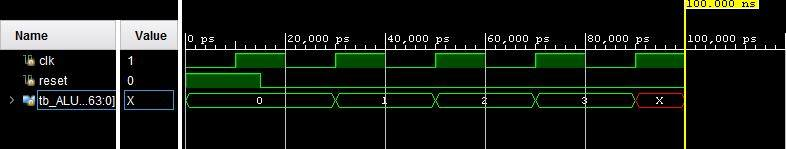
\includegraphics[width=\textwidth, keepaspectratio]{Lab9Instr.jpg}

  \centering
  \caption{Instruction Set 2: GitHub Instructions}
    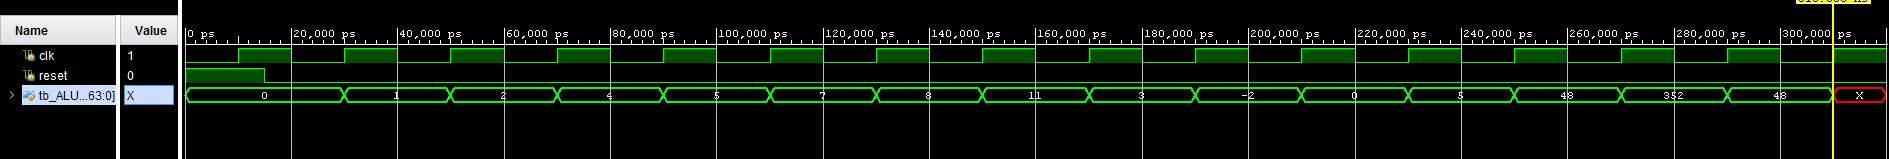
\includegraphics[width=\textwidth, keepaspectratio]{GitHubInstr.jpg}

    \centering
      \caption{Instruction Set 3: Our 12 RISC-V Instructions}
    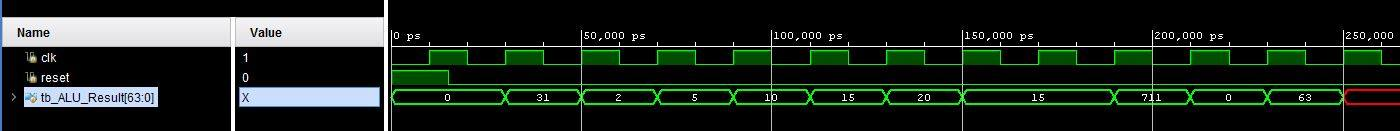
\includegraphics[width=\textwidth, keepaspectratio]{Um12Instr.jpg}
\end{figure}

\subsection{FPGA Implementation} 
Implementation of the 12 instructions we created onto the FPGA. The following images are of two instructions.

\begin{figure}[htp]
    \centering
    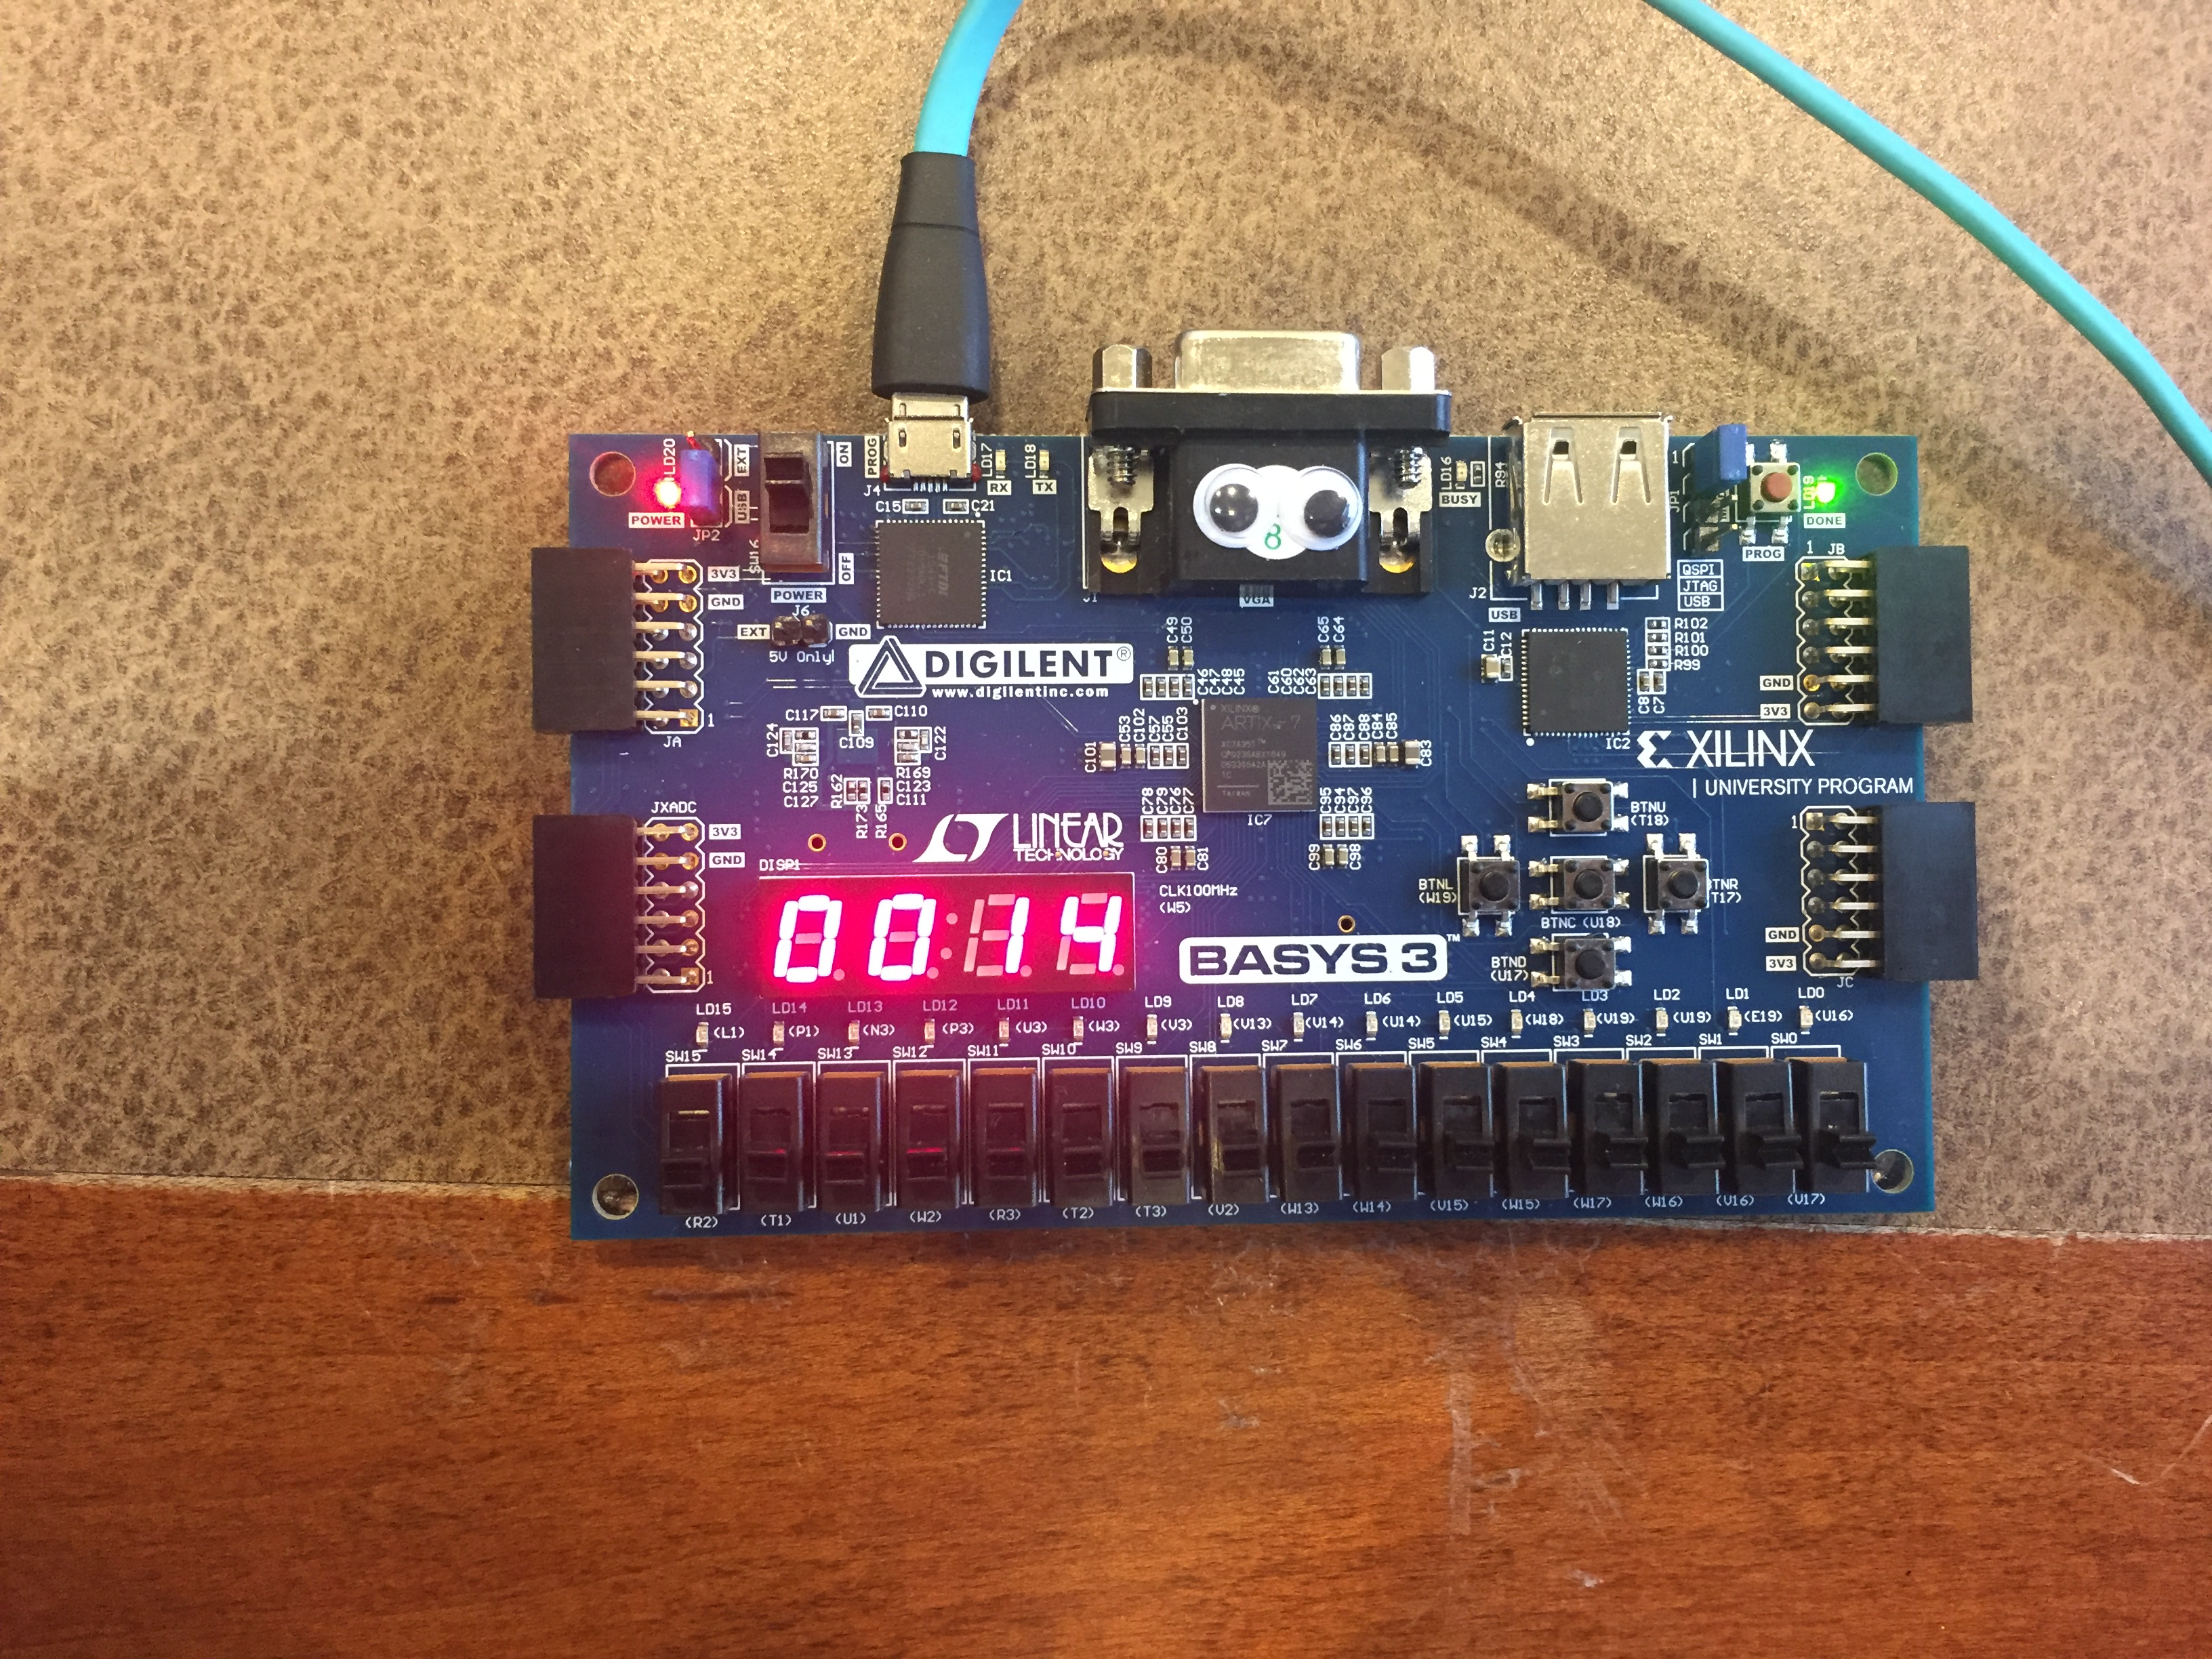
\includegraphics[width=\textwidth, keepaspectratio]{addi_r2,r1,05.JPG}
    \centering
    \caption{Instruction = 32'h00128533; \\32’b0000000 00001 00101 000 01010 0110011; ADD R10, R5, R1 (R10 = 20)}
    \label{fig:my_label}
\end{figure}
\begin{figure}[htp]
    \centering
    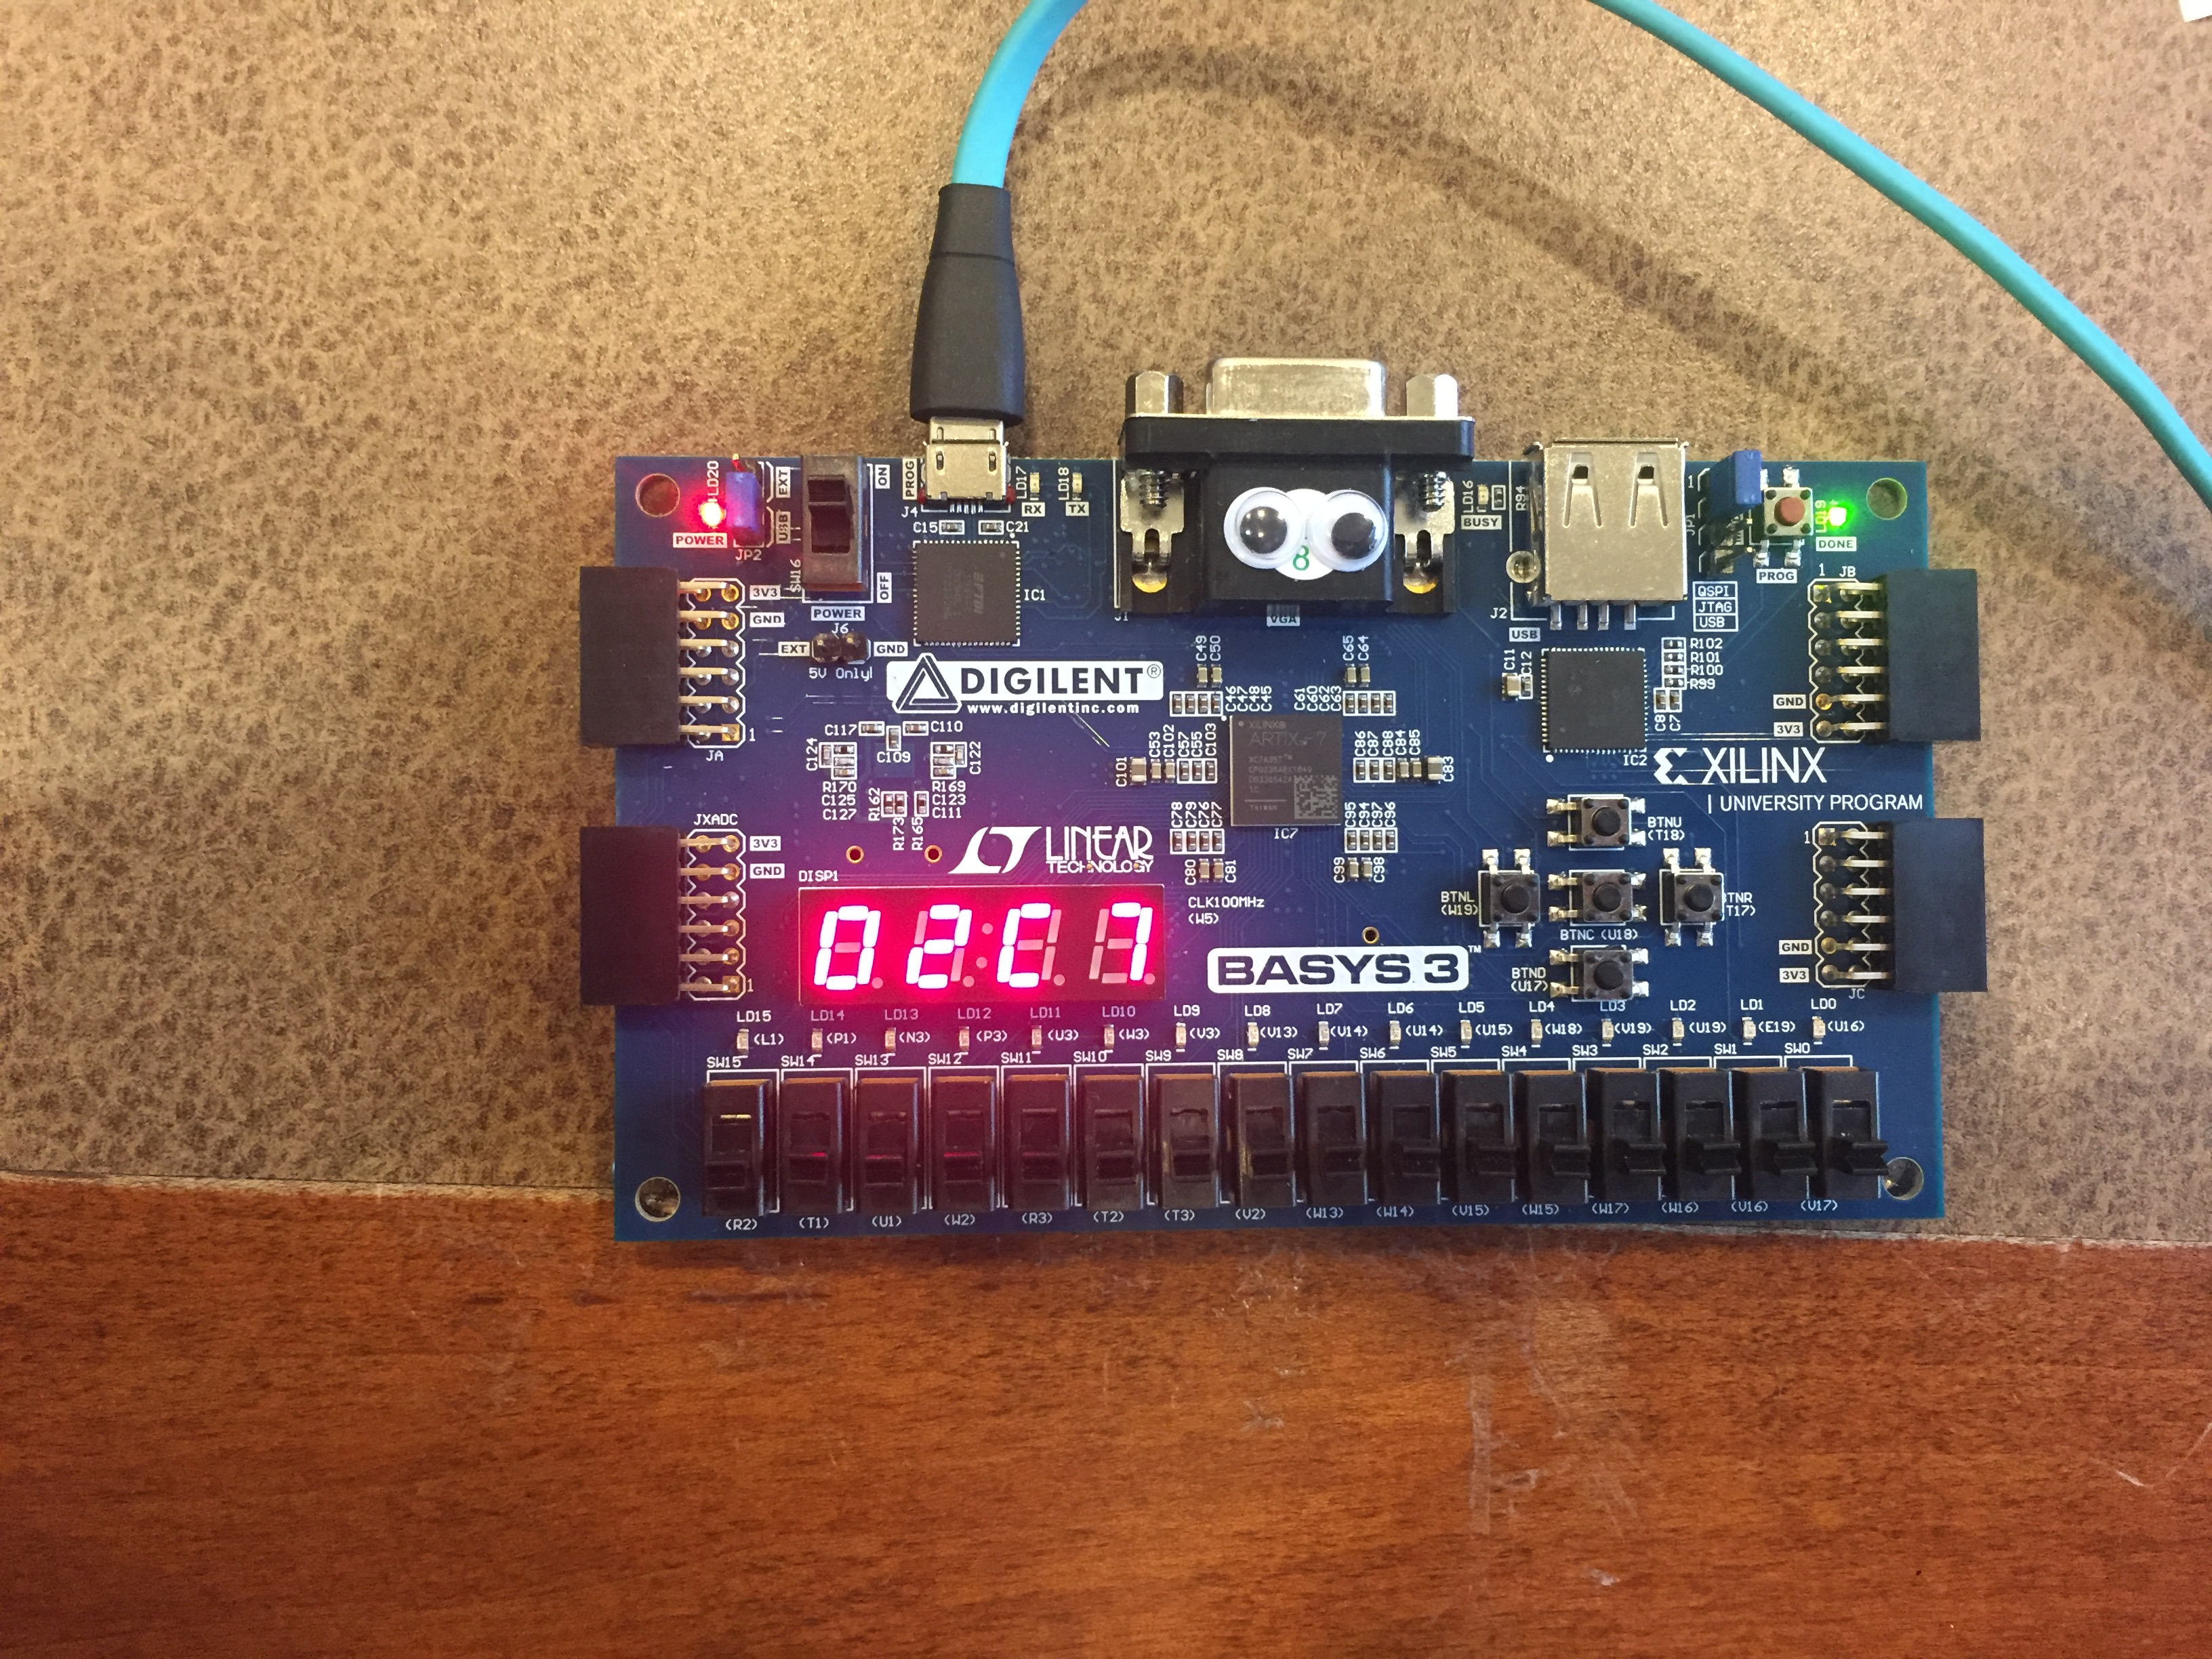
\includegraphics[width=\textwidth, keepaspectratio]{or_r12.JPG}
    \centering
    \caption{Instruction = 32'h00516633; \\32’b0000000 00101 00010 110 01100 0110011;   OR R12, R2, R5 (R12 = R2 OR R5)}
    \label{fig:my_label}
\end{figure}

\end{document}
